\begin{enumerate}
\item Il s'agit d'une application immédiate des propositions relatives aux opérations sur les fonctions admettant des limites finies.
\item  La fonction racine carrée est continue dans $\R^+$. D'apr\`{e}s les propri\'{e}t\'{e}s de la fonction partie enti\`{e}re, elle est réglée. Les points de discontinuit\'{e}s de $f_r$ sont les $x$ tels que $r\sqrt{x}$ soit entier c'est \`{a} dire tous les $x$ de la forme
\begin{displaymath}
 \frac{n^{2}}{r^{2}} \text{ avec } n\in \N
\end{displaymath}
Pour chaque point de discontinuité, le saut est $+1$.
\item  La question pr\'{e}c\'{e}dente permet de former les discontinuit\'{e}s de chaque fonction : 
\[
\renewcommand{\arraystretch}{1.6}
\begin{tabular}{c|ccc|c}
fonction & discontinuités & & & coefficient\\ \hline
$f_{a}$ & 2 & 8 &  &2\\ \hline
$f_{b}$ & $\dfrac{1}{(\sqrt{2}-1)^{2}}$ &  & &-1 \\ \hline
$f_{c}$ & 1 & 4 & 9 &-1
\end{tabular}
\]
On range les points de discontinuité par ordre croissant :
\begin{displaymath}
1 < 2 < 4 < \frac{1}{(\sqrt{2}-1)^{2}} < 8 < 9 
\end{displaymath}
Entre deux discontinuit\'{e}s, la fonction $g$ est constante. \`A chaque travers\'{e}e d'une discontinuit\'{e}, la fonction $f_{r}$ correspondante augmente de 1. On obtient le graphe de $g$ en partant de l'origine et en reportant les sauts en tenant compte du signe et du coefficient (voir figure \ref{fig:Cdiscont_1}).
%insertion du graphe
\begin{figure}[h!t]
   \centering
   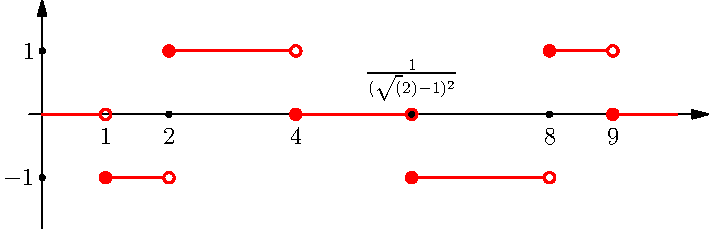
\includegraphics{Cdiscont_1.pdf}
   \caption{graphe de $g$}
   \label{fig:Cdiscont_1}
\end{figure}

\item  Par d\'{e}finition d'une partie enti\`{e}re : 
\begin{displaymath}
r\sqrt{x}-1<f_{r}(x)\leq r\sqrt{x} 
\end{displaymath}
En combinant ces in\'{e}galit\'{e}s avec les coefficients pour les trois fonctions, il vient : 
\begin{align*}
2(a\sqrt{x}-1)-b\sqrt{x}-c\sqrt{x} < &g(x)<2a\sqrt{x}-(b\sqrt{x}-1)-(c\sqrt{x}-1) \\
(2a-b-c)\sqrt{x}-2 < &g(x)<(2a-b-c)\sqrt{x}+2
\end{align*}
Mais $2a-b-c=0$ et $g(x) \in \Z$ donc $-2<g(x)<2$ entra\^{\i }ne $g(x)\in \{-1,0,1\}$.

\item L'ensemble des points de discontinuité de $g$ est l'union des ensembles de points de discontinuité de $f_a$, $f_b$, $f_c$. Ces ensembles sont (d'après la question 2.) :
\begin{align*}
 \left\lbrace 2p^2,p\in \Z\right\rbrace & & 
\left\lbrace \frac{q^2}{3-2\sqrt{2}},q\in \Z\right\rbrace & &
\left\lbrace r^2,r\in \Z\right\rbrace   
\end{align*}
Ils sont deux à deux disjoints car $\sqrt{2}$, $\frac{3}{2}-\sqrt{2}$ et $\sqrt{2}-1$ sont irrationnels. On peut alors appliquer le résultat de linéarité du saut démontré en question 1. On en déduit qu'en un point de discontinuit\'{e} de $f_{a}$, le saut est $+2$ alors qu'en un point de discontinuit\'{e} de $f_{b}$ ou $f_{c}$ le saut est $-1$.

\item  Raisonnons en distinguant plusieurs cas et en exploitant le fait que $g$ ne prend que les valeurs $-1$, $0$ et $1$ avec des sauts $+2$ ou $-1$ et qu'aucun des trois ensembles de discontinité n'est majoré (il existe donc des discontinuités de chaque type après un réel arbitraire):
\begin{itemize}
\item  Si $g(A)=-1$, le premier saut de discontinuit\'{e} est forc\'{e}ment $+2$. La fonction prend alors la valeur $+1$. Le saut suivant est obligatoirement $-1$ et la fonction $g$ prend alors la valeur $0$.

\item  Si $g(A)=0,$ le premier saut de discontinuit\'{e} est forc\'{e}ment $-1$. La fonction prend la valeur $-1$ et on se retrouve dans le cas pr\'{e}c\'{e}dent.

\item  Si $g(A)=+1$, le premier saut de discontinuit\'{e} est forc\'{e}ment $-1$. La fonction prend la valeur $0$ et on se retrouve dans le cas pr\'{e}c\'{e}dent.
\end{itemize}
La fonction $g$ prend donc les trois valeurs sur tout intervalle $\left[A,+\infty \right[$.
\end{enumerate}